%----------------------------------------------------------------------------------------
%	Chapter 1
%----------------------------------------------------------------------------------------

% To have just one problem per page, simply put a \clearpage after each problem

\section{Aim}
The objective of this project is to predictive the latitude and longitude for a set of test users, given their social friends network and other metadata information as detailed below:

\begin{itemize}
\item A graph of social network, as a tab-delimited file with each line having two user IDs.
\item A training dataset is a csv file of userIds, top 3 hours in GMT where the user make the maximum number of posts during the day and the total number of posts. The training data also contains the lat and lon.
\item The test dataset contains all the fields available in the train dataset except for the latitude and the longitude.
\end{itemize}

\section{Method \& Results}


\begin{itemize}
\item Clean up data by removing invalid hours (hour  greater than 24)
\item Transform features as shown below

\begin{footnotesize}
\begin{tabular}{ll}

\toprule
Features & Description \\
\midrule
EarliestHr & min(hour1,hou2,hour3) \\
LatestHr & max(hour1,hour2,hour3) \\
TotalBestHr & EarliestHr + LatestHr) \\
FriendsDistance & abs (myearliestHr - myfriendsEarliestHr) +  abs(mylatestHr - my friendsLatestHr) \\
closestFriendLat & Latitude of friend with min(friendsDistance) \\
closestFriendLon & Longitude of friend with min(friendsDistance) \\
\midrule
 & \tiny{*Friend Indicates depth 1 friends in graph.}  \\
 & \tiny{**When no friends lat lon is available , the entire data set is assigned as friends} \\
\bottomrule
\label{tab:features}
\end{tabular}
\end{footnotesize}

\item Split the training data into a test and training set and identify best model by applying set of algorithms show below\ref{tab:Algorithms}


\begin{footnotesize}


\begin{tabular}{lll}

\toprule
Model & Formula & RMS \\
\midrule
Linear regression & lat\\~hour1+hour2+hour3, lon\~hour1+hour2+hour3 & 80 \\
SVM for regresssion & lat\~hour1+hour2+hour3, lon\~hour1+hour2+hour3 & 80 \\
Linear regression & lat\~closestFriendLat, lon\~closestFriendLon & 25.9 \\
Bagging with regression & lat\~closestFriendLat, lon\~closestFriendLon, bags=50, ns=n/3, combined=weighted & 26.5 \\
knn regression & lat\~closestFriendLat, lon\~closestFriendLon, k=5 & 61 \\
Bagging with regression & lat\~closestFriendLat, lon\~closestFriendLon + totalBestHr, bags=50, ns=n/3, weighted & 35 \\

\bottomrule

\label{tab:Algorithms}
\end{tabular}


\end{footnotesize}

\end{itemize}

\subsection{Results}
The rms scores  for the final set of 3 best algorithms run on training data sampled into train and test set is shown below

\begin{footnotesize}
\begin{tabular}{llllllllll}

\toprule
 & LR Lat & LR Lon & LR Avg & Bagged Lat & Bagged Lon & Bagged Avg & KnnR Lat & Knn  Lon & KnnR Avg \\
\midrule
1 & 12.11986529 & 39.81742322 & 25.96864425 & 12.33299222 & 40.9195119 & 26.62625206 & 22.72443501 & 61.59112081 & 42.15777791 \\
2 & 12.11978357 & 39.82049648 & 25.97014002 & 12.29019479 & 40.91197876 & 26.60108678 & 23.31113756 & 62.54626114 & 42.92869935 \\
3 & 12.1201144 & 39.82062573 & 25.97037007 & 12.30435766 & 40.95575127 & 26.63005446 & 22.58698289 & 62.53609033 & 42.56153661 \\
4 & 12.11989517 & 39.81262501 & 25.96626009 & 12.31286676 & 40.87628583 & 26.5945763 & 21.66892361 & 62.8944826 & 42.28170311 \\
5 & 12.1200593 & 39.8158162 & 25.96793775 & 12.2987158 & 40.866485 & 26.5826004 & 22.55446468 & 63.22945695 & 42.89196081 \\
6 & 12.11964583 & 39.81020173 & 25.96492378 & 12.2908289 & 40.88872642 & 26.58977766 & 22.18445203 & 62.72836326 & 42.45640764 \\
\bottomrule
\end{tabular}
\end{footnotesize}



\section{Discussion}

\subsection{Features}
The features available in the data are top 3 hours of the day during which the user posts the maximum number of posts, the total posts per day and  a network of the user's friends. In order to estimate the latitude and the longitude, the set of features of features that best predict these output variables must be identified.  Using features that do not correlate with the output can result in poor prediction.  In order to  identify a possible subset of features that are the best predictors, we could use an intuitive approach of applying  domain knowledge or a more formal approach such as computing correlation or mutual information \cite{Guyon2003}.




\subsection{Feature Selection}
In this project, we have used domain knowledge and visualisation techniques to identify the best predictors.  Intuitively, in most cases, the location of our friends are good indicators of where we are. The next possible indicator is using the hours, given it all in GMT, to calculate longitude as show in \ref{fig:featureHour}. 


\begin{center}
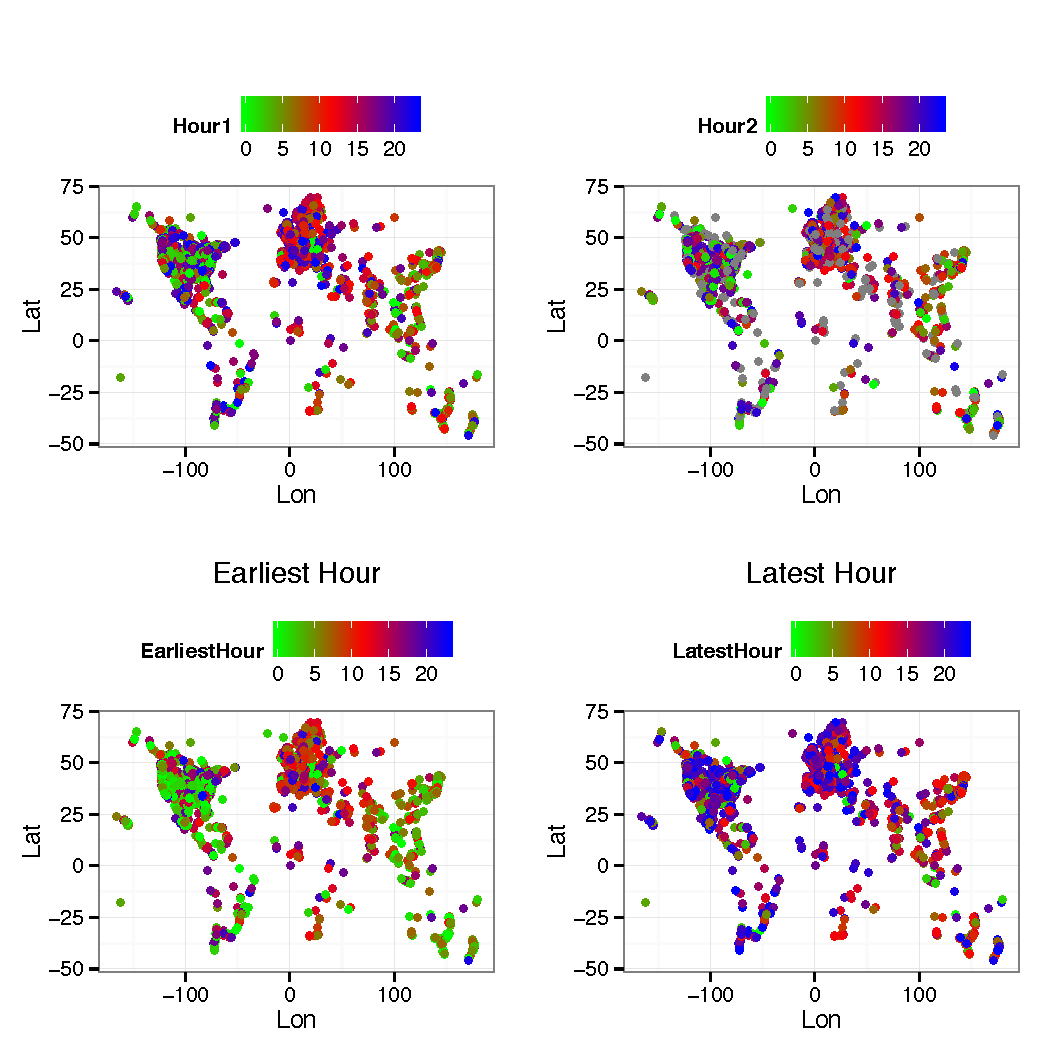
\includegraphics[width=0.75\columnwidth, height=.5\columnwidth]{figures/featurePlot.pdf} % Example image
\label{fig:featureHour}
\end{center}

\subsection{Feature Transformation}
Although the hours directly do not seem to indicate the longitude, transformating hour1, hour2 and hour2 into earliest and latest hours (min(hour1, hour, hour) \& max (hour,hour2,hour3) are able broadly identify 3 zones , the Americas, Europe \& Africa and AsiaPacific. Moreover, most common model do not accept the  friends graph directly and hence the friends latitude and longitude have been transformed to closest friends latitude and longitude.

\subsection{Algorithms}
We have attempted to use linear regression, bagging, Knn and SVM regression models. Svm tended to be slower than linear regression. Bagging had lightly higher RMSE scores  to linear regression with  in training data, but in the final test data, bagging score ended up lower. This could possibly be explained the ability of bagging to average out noisy errors, the test data set possibly was noisier that the training data.
Knn Regression performed poorly, possibly due to parameter or formula errors. 

\subsection{Overfitting and Underfitting}
The average score  RMSE of 25 is low in bagging and regression in the train runs, indicating that the model is not under fitted. To ensure that the model is not over fitted , we ran the experiment several times using the first 100 rows in the training data as the test set, and by by sampling  10000 from the remaining data. The average RMSE score remained almost consistent despite varying the data for the model (as shown in results table). The low variance in RMSE scores  indicates the model is not overfitted. 

\section{Conclusion}
\begin{itemize}
\item Feature selection is critical to developing a good model.
\item Linear regression and SVR (SVM for regression) had similar results in this project, except that SVM was 10 times slower than linear regression which can be explained by the polynomial time that SVM takes.
\item Bagging with linear regression provides better results than a single linear regression predictor by neutralising the errors caused by noisy data.
\item The rms scores for latitude is much lower than that for longitude, possibly explained by the smaller range of available values for latitude.
\end{itemize}

\section{Further Improvements}
\begin{itemize}
\item Use formal approaches such as Pearsons correlation and mutual information to identify features that can improve the predictor variables.
\item Try other regression models such as random forests , neural network to further improve the model.
\item Averaging the results of several good models might also improve the results
\end{itemize}
